\subsection{Graphs for community detection}

Before we start, we need to make sure we understand some basic notions about graphs:

\begin{itemize}
    \item \textbf{Degree of node}: Number of neighbors of a node. In directed graphs, we have in and out degree
    \item \textbf{Diameter of a graph:} Length of the longest shortest path
\end{itemize}

There are a number of ways to construct graphs from data:

\begin{itemize}
    \item k-NN: Connect every point with the closest $k$ items
    \item $\varepsilon$-neighbourhood: Connect all points within $\varepsilon$ distance
    \item Fully-connected graph: Choose a distance $dist$, then connect any point to any other point. The weight of each edge $(u, v)$ corresponds to $(1 - dist)$ between $u$ and $v$
\end{itemize}

\subsection{Spectral Graph Theory}
    We want to study the adjacency matrix of a graph using linear algebra. We will identify connections between ``spectral properties'' of such a matrix and structural properties. These include properties such as 
    \begin{itemize}
        \item Degree
        \item Centrality
        \item Communities
        \item Flows
    \end{itemize}

If our graph is undirected, then the adjacency matrix is symmetric. By the spectral theorem, we know that eigenvectors are real and orthogonal.

\subsubsection{The adjacency matrix}
    We can think of $A$ as an operator of an undirected graph $G$. 
    
    Let $x \in \R^n$ with components $(x_1, \dots, x_n)$, then we can think of it as a label/value of each node of $G$. 
    
    What then is the meaning of 
    \m{
        \mat{a_{11} & \dots & a_{1n} \\
            \vdots & & \vdots \\
            a_{n1} & \dots & a_{nn}
        } \mat{x_1 \\ \vdots \\ x_n} = \mat{y_1 \\ \vdots \\ y_n}
    }
    It turns that it equals $y_i = \sum_{(i, j) \in E}{x_j}$, or entry $y_i$ is the sum of labels $x_j$ of neighbours of $i$. So the $y$ contains for each node, the sum of all its neighbours. If we apply this multiple times, we then keep propagating labels throughout the network iteratively. 
    
    Consider that this could be written as  \m{
        Ax = \lambda \cdot x
    }
    Which naturally gives way to considering eigenvalues and eigenvectors. 
    
    \subsubsection{The essence of spectral graph theory}
        In spectral graph theory, we want to analyse the spectrum of a matrix representing a graph $G$. This spectrum is
        
        \m{\Lambda = \set{\lambda_1, \dots, \lambda_n}}
        Ordered by 
        \m{
            \lambda_1 \geq \lambda_2 \geq \dots \geq \lambda_n
        }
        Recall the definition of eigenvalues and eigenvectors. If $\lambda \in \C$ is an eigenvalue if there exists a vector $x \in \C^n, x \neq 0$ such that 
        \m{
            Ax = \lambda x
        }
        Or 
        \m{
            (A - \lambda I)x = 0
        }
        So $A$ has $n$ eigenvalues.
        
        But first, we need to understand what it means for a matrix to be symmetric.
    
    \subsubsection{Prerequisites}    
    
        A matrix $A$ is symmetric if
        \begin{itemize}
            \item All eigenvalues are $\lambda \geq 0$
            \item $x^T Ax \geq 0$ for all $x$ (PSD)
            \item $A = N^TN$
        \end{itemize}
        
        Let us look at an example to illustrate eigenvalues and eigenvectors of a graph $G$. Suppose we have a $d$-regular graph, where each vertex has degree $d$. $y_i$ is the inner product of row $i$ and $x$. Suppose $A$ is the adjacency matrix, then we know that for each row, $d$ entries will have value $1$. If $x = (1, 1, \dots, 1)$, then $Ax = (d, d, \dots, d)$. What is $\lambda$ then? it is $\lambda = d$.
        
        Another example is a graph with two components. Say each component is $d$-regular. Let us say that $x$ contains $1$s on A and $0$ on B. If $x' = (1, \dots, 1, 0, \dots, 0)$ then $Ax' = (d, \dots, d, 0, \dots, 0$ for $x'$ being the $A$ vector. In both cases the corresponding $\lambda = d$. 
        
        If we have a connected graph, then we know that $x_1 = (1, \dots, 1)$ is an eigenvector. Since eigenvectors are orthogonal, then the components of $x_2$ must sum to $0$. That is because $x_1^T x_2$ must be $0$ for them to be orthogonal, and since $x_1$ has all $1$ in the entries, then they must sum to $0$. 
        
        Consider the matrix $A$ which is real and symmetric. The eigenvalues $\lambda_1, \dots, \lambda_n$ ordered by decreasing size. 
        
        \begin{defi}
        Variational characterization of eigenvalues.
        \begin{enumerate}
            \item \m{\lambda_n = \min_{x \neq 0}{\frac{x^T Ax}{x^T x}} = \min_{x \neq 0}{\frac{\sum_{ij}A_{ij}x_ix_j}{\sum_{i}x_i^2}}}
            \item \m{
                \lambda_{n-1} = \min_{x \neq 0, x^T x_1 = 0}{\frac{x^T Ax}{x^T x}}
            }
            \item \m{
                \lambda_1 = \max_{x \neq 0}\frac{x^T Ax}{x^T x}
            }
        \end{enumerate}
        And so on for other eigenvalues
        \end{defi}
        
\subsubsection{Matrix representations}
    There are a couple of important matrix representations that we need to understand. 
    \begin{itemize}
        \item The \textbf{Degree Matrix} or $\Delta$ is an $n \times n$ diagonal matrix where $\Delta_{ii}$ is the degree of node $i$. 
        \item The \textbf{Laplacian Matrix} or $L$ is an $n \times n$ symmetric matrix. It is defined as $L = \Delta - A$
    \end{itemize}
    $L$ has trivial eigenpair $x = (1, \dots, 1)$. Because $Lx = 0$ with $\lambda = \lambda_n = 0$. However, there are a few important properties to consider. The eigenvalues are non-negative real numbers, and the eigenvectors are real and orthogonal. 
    
    Furthermore there are also a few variations of the Laplacian
    \begin{itemize}
        \item Unnormalized Laplacian: $L = \Delta - A$
        \item Normalized (Symmetric) Laplacian: $L^s = \Delta^{- \frac{1}{2}}L \Delta^{-\frac{1}{2}}$
        \item Asymmetric (Random Walk) Laplacian: $Lâ = I - \Delta^{-1}A$
    \end{itemize}
    
\subsubsection{Spectral graph analysis}
    For our Laplacian $L = \Delta - A$, we have that
    \m{
        x^T Lx = \sum_{(u, v) \in E}{(x_u - x_v)^2}
    }
    Wherre $x_u$ is the coordinate of the eigenvector $x$ corresponding to the vertex $u \in V$ (Remember $Lx = \lambda x)$
    Here we can think of the eigenvector $x$ as a one-dimensional embedding that maps vertices to the real number line.
    
    
\subsection{Spectral clustering}
    We are interested in using this theory for community detection. We will work with undirected and unweighted graphs and use this theory to find communities (clusters). 
    
    Consider the problem of graph partitioning. For example, in bi-partitioning, we divide vertices into two disjoint groups $A$ and $B$. We want to define what it means to have a good partition of $G$, and we want to efficiently identify such partitions. 
    
    A good partition is one that maximises the number of within-group connections, and minimizes the number of between-group connections. 
    
    We can express partitioning objectives as a function of the ´´edge cut'' of the partition. A cut is a set of edges with only one vertex in a group. \m{
        W(A, B) = \sum_{i \in A, j \in B}a_{ij}
    }
    We want to minimise this quantity. However, this does not necessarily maximise the number of in-group connections. We can therefore look at the ratio-cut criteria (which is a form of normalized cut). This is the connectivity between groups relative to the density of each group 
    \m{
        J_{rc}(C) = \frac{W(A, B)}{|A|} + \frac{W(A,B)}{|B|}
    }
    where $C = \set{A, B}$. This is better, but computing optimal cuts is NP-Hard. 
    
    Returning to eigenvalues for a second. We know that \m{
                \lambda_{n-1} = \min_{x \neq 0, x^T x_1 = 0}{\frac{x^T Ax}{x^T x}}
            }
    Look at the numerator and consider what $x^T Ax$ means. It is equal to $\sum_{ij \in E}(x_i - x_j)^2$. 
    
    We know that $x$ is a unit vector. We know that $x$ is orthogonal the first eigenvector $(1, \dots, 1)$. 
    
    We want to assign values $x_i$ to nodes $i$ such that few edges cross $0$. We want $x_i$ and $x_j$ to subtract each other. Thus we want 
    
    \m{
        \lambda_{n-1} =  \min \frac{\sum_{i, j \in E}(x_i - x_j)^2  }{\sum_i x_i^2}
    }
    Where the unit vector property of $x$ gives $\sum_i x_i^2 = 1$
        
    \begin{center}[h]
        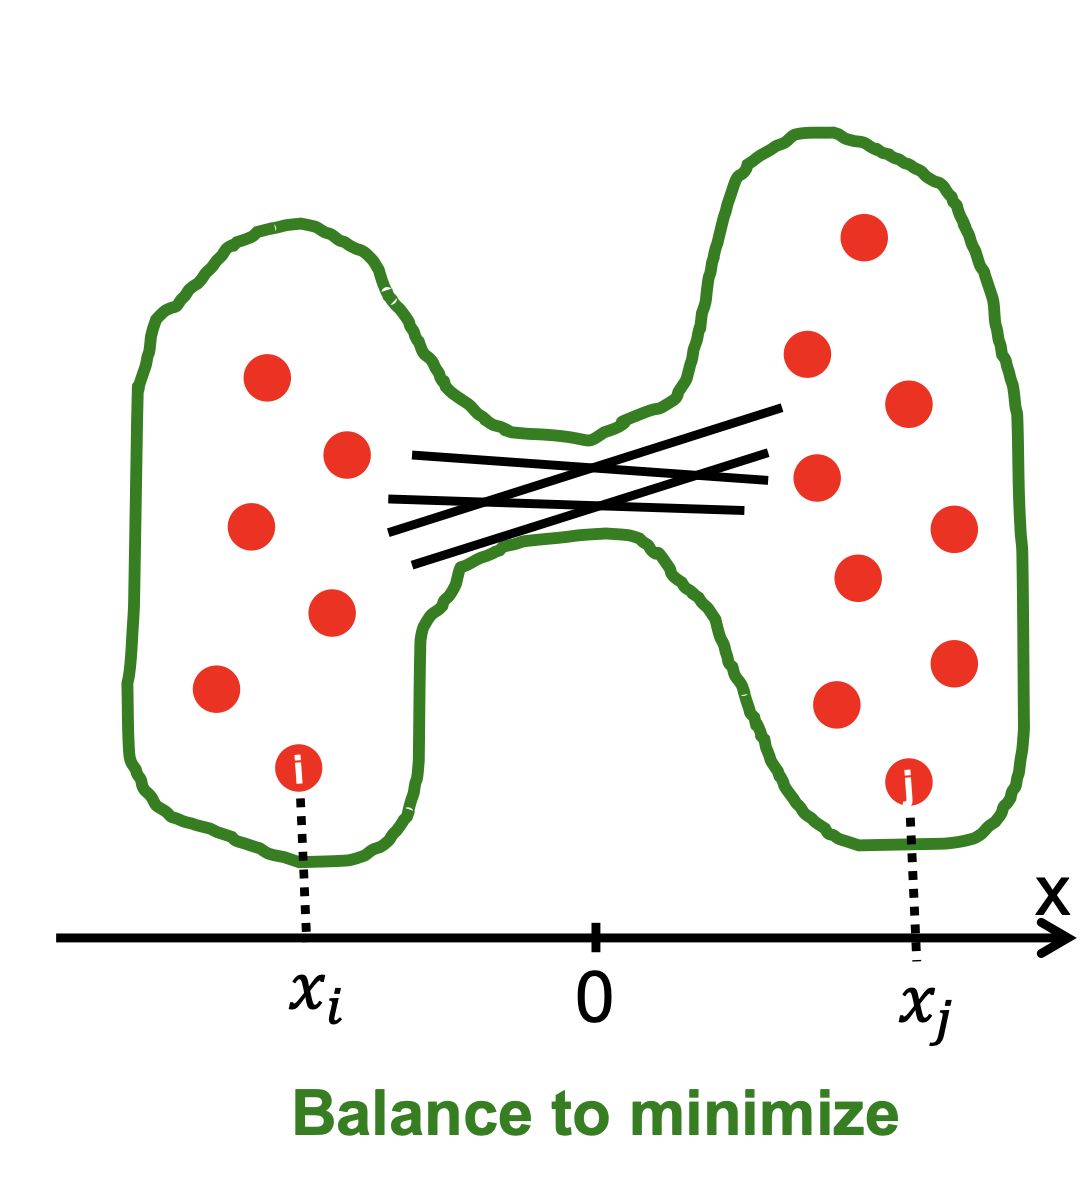
\includegraphics[width=0.5\textwidth]{images/balance.png}
    \end{center}
    
    This means that in order to find the optimal cuts, we can do the following:
    
    Express a partition $(A, B)$ with vector 
    \m{
    x_i = \begin{cases}
        +1 & \text{if } i \in A \\
        -1 & \text{if } j \in B
    \end{cases}
    }
    We can minimize the cut of the partition by finding a non trivial vector $x$ that minimizes
    \m{
        \arg \min f(x) = \sum{(x_i - x_j)^2}
    }
    Subject to $x \in [-1, 1]^n$. We cannot solve this directly, but we can allow $x$ to take any value instead. 
    
    \begin{center}[h]
        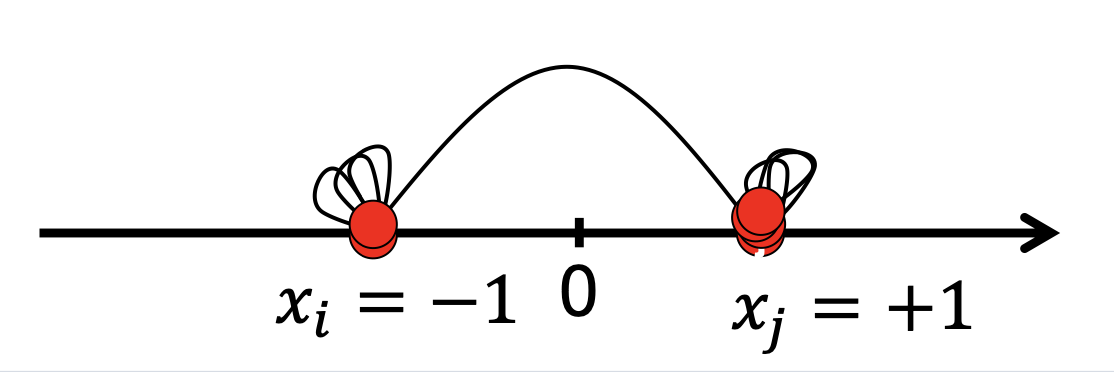
\includegraphics[width=0.5\textwidth]{images/lr.png}
    \end{center}
    
    This brings us to \emph{Rayleigh's Theorem}. Consider \m{
        \min_{x \in \R^n}f(x) = \sum_{i,j \in E}{(x_i - x_j)^2} = x^T L x
    }
    The minimum value of $f(x)$ is given by the 2nd smallest eigenvalue $\lambda_{n-1}$ of the Laplacian $L$. $x = \arg \min_x f(x)$. The optimal solution for $y$ is given by the corresponding eigenvector $x$, referred to as the Fiedly vector. 
    
\subsubsection{Spectral Clustering algorithms}
Spectral Clustering algorithms have $3$ basic stages. 
\begin{itemize}
    \item \textbf{Preprocessing:} Construct a matrix representation of the graph
    \item \textbf{Decomposition:} Compute the eigenvalues and eigenvectors of the matrix. Map each point to a lower-dimensional represenation based on one or more eigenvectors
    \item \textbf{Grouping:} Assign points to two or more clusters, based on new representation
\end{itemize}

The \emph{Spectral Partitioning Algorithm} does exactly that. In the decomposition phase, it maps vertices to corresponding components of $\lambda_2$ and its vector. But how do we find the new clusters? We can sort the components of the new $1$-dimensional vector. We could split at $0$ or the median value. Consider for example (First column is index) that the vector of $\lambda_2$ is
\m{
\mat{1 & 0.3 \\
    2 &  0.6 \\
    3 & 0.3 \\
    4 & -0.3 \\
    5 & -0.3 \\
    6 & -0.6}
}
Then we could split them into $A = \set{1, 2, 3}, B = \set{4, 5, 6}$. We could also do something more expensive and try to minimize normalized cuts in 1D.

    \begin{center}
        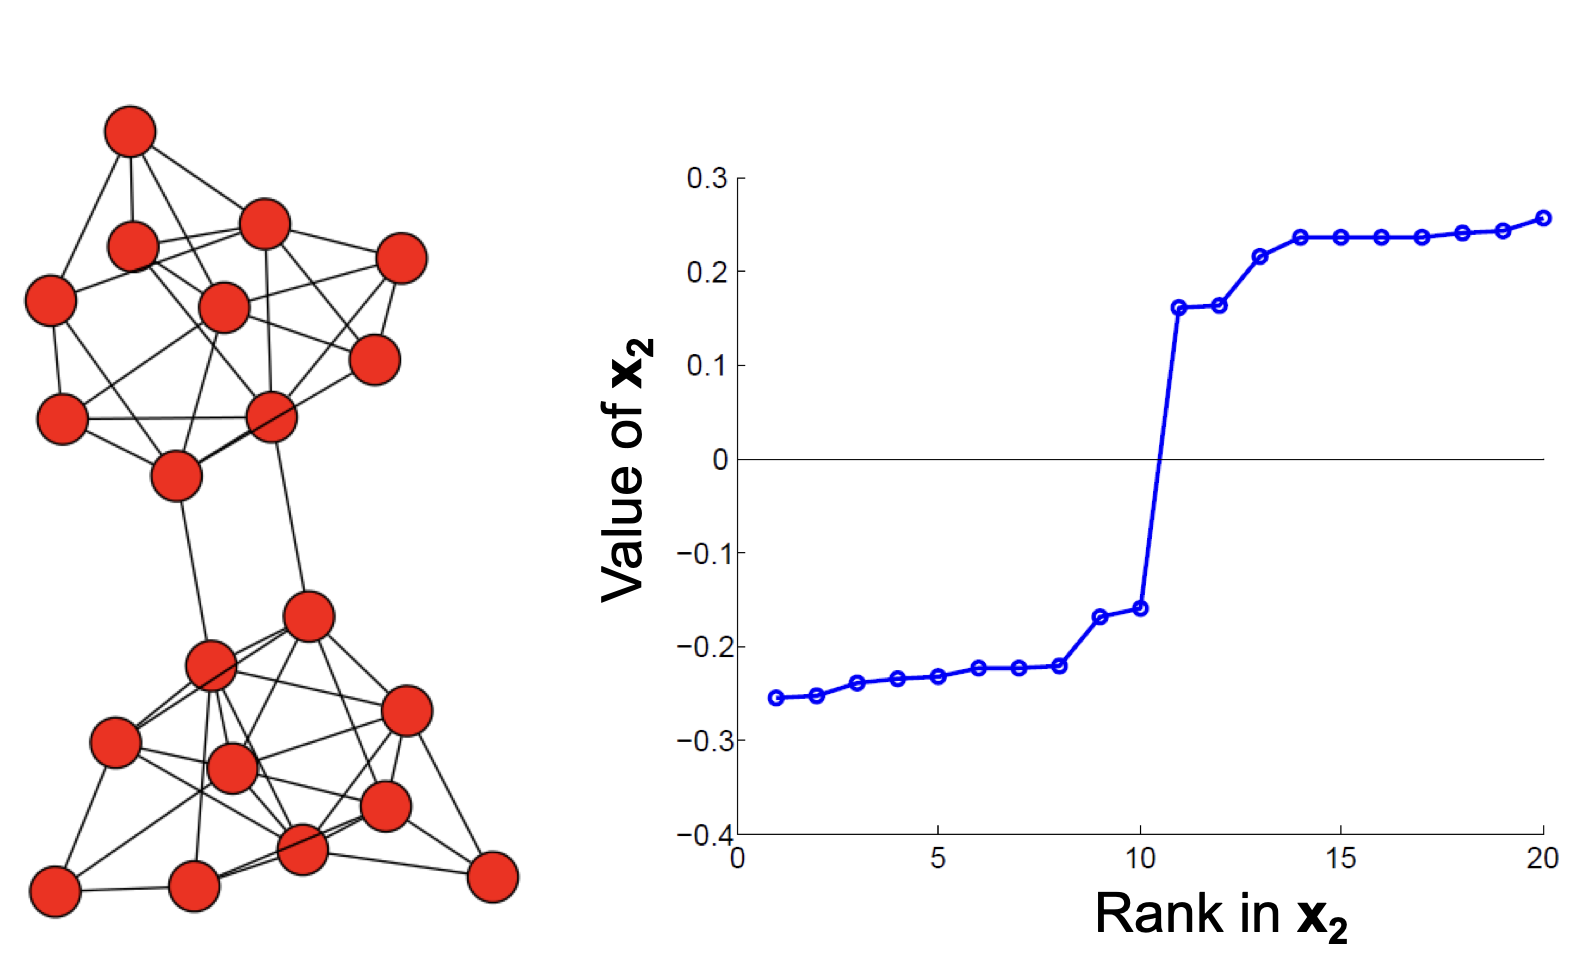
\includegraphics[width=0.5\textwidth]{images/valueverussrank.png}
    \end{center}
Not only do we see these kinds of behaviours on these plots, but for graphs with multiple clusters, we see these clusters apparent when we plot value versus rank.
    
    
\subsubsection{$k$-way spectral clustering}
    If we want $k$ clusters, then we can use recursive bi-partitions, but this is expensive and unstable. We can also do something better, and use multiple eigenvectors. We can build a reduced space from these multiple eigenvectors. 
    
    This has the following properties:
    \begin{itemize}
        \item it approximates the optimal cut ($k$-way normalized cut)
        \item It emphasises cohesive clusters. It increases unevenness in the distribution in the data. The associations between similar points are amplified. The data begins to approximate clustering
        \item It gives us a well-seprated space. It transforms data to a new embedded space consisting of $k$ orthogonal basis vectors
        \item Multiple eigenvectors prevent instability caused by information loss
    \end{itemize}
    If we take the objective of Kernel $k$-means, then it looks a lot like it. 
    
    The advantages of Spectral Clustering is
    \begin{itemize}
        \item Clusters can have arbitrary shapes and size (e.g not convex)
        \item Efficient in normal (sparse) graphs
        \item Robust to noise and is theoretically grounded and well-connected to graph properties
    \end{itemize}
    The disadvantages are
    \begin{itemize}
        \item Inefficient on dense groups ($O(n^3)$ worst case)
        \item Need to provide number of clusters
    \end{itemize}
    
\subsection{Modularity}
    Communities are sets of tightly connected vertices. We can define modularity $Q$ as a measure of how well a network is partitioned into communities, given a partitioning of the network into groups $s \in S$. 
    \m{
        Q \varpropto \sum{s \in S} [\text{number of edges within group $s$} - \text{expected number of edges within group $s$}]
    }
    We need a model to determine these values. 
    
    Given a real $G$ with $n$ vertices and $m$ edges, construct a rewired graph $G'$. It has the same degree distribution but random connections. We can consider it a multigraph (multiple edges for same pair of nodes). We can then ask: What is the expected number of edges between the nodes?
    
    The probability that one node is $i$ and the other is $j$ is \m{
        p_{rs} = \frac{d_i d_j}{2m^2}
    }
    The expected number of edges between nodes $i$ and $j$ of degrees $k_i, k_j$ is $2m \cdot p_{rs} = \frac{k_i k_j}{2m^2}$
    Thus the expected number of edges in multigraph $G'$ is \m{
    \frac{1}{4m}2m \cdot 2m = m
    }
    
    Hence the modularity of a partion $S$ of $G$ is 
    \m{
        Q(G, C) = \frac{1}{2m}\sum_{c \in C}\sum_{i \in c}\sum_{j \in c} (a_{ij} - \frac{d_i d_j}{2m})
    }
    Note that we normalize, so values are in the range $[-1, 1]$. It is positive if the number of edges within groups exceeds the expected number. If it is between $0.3$ and $0.7$ that means there is significant community structure. 
    
    Note that modularity cannot be $1$ and it is NP-hard to optimise modularity directly. 
    
    Say we want to maximise $Q$
    
    \m{
        Q = \sum_{i}(u^T c)^2 \beta_i
    }
    Since the largest eigenvalue corresponds to $u_1$ and given the fact that other eigenvectors are orthogonal, we would like to choose at least $s$ that maximises $u_i^T c \rightarrow u_i, c$ are parallel. But $s_i$ must be $+1, -1$. So we maximise $u_1 c$, the projection of $s$ along $u_1$. To do this, we choose $s_i = 1$ if $u_1 \gt$, and $-1$ otherwise. 
    
    A greedy improvement is to repeat finding a vertex that would yield the largest modularity increase if it were moved into a different community AND that has not yet been moved. 
    
    Modularity clustering has the following advantages
    \begin{itemize}
        \item Clusters can have arbitrary shape and size, i.e clusters are not restricted to have convex shapes
        \item Efficient in normal sparse graphs
        \item Robust to noise
    \end{itemize}
    The disadvantages are
    \begin{itemize}
        \item Inefficient on dense graphs with $O(n^3)$ in the worse case
        \item Need to provide number of clusters, and it favours small communities
    \end{itemize}
    
\subsection{Girvan-Newman}
    The Girvan Newman method is a divise hierachical clustering based on the notion of \emph{edge betweenness}. This is the number of shortest paths that cross over the edge. 
    
    The algorithm repeats (until no more edges are left) calculating the betweenness of edges. It removes edges with the highest betweenness and then recomputes. This gives a hierarchical decomposition of the network. 
    
    \begin{center}
        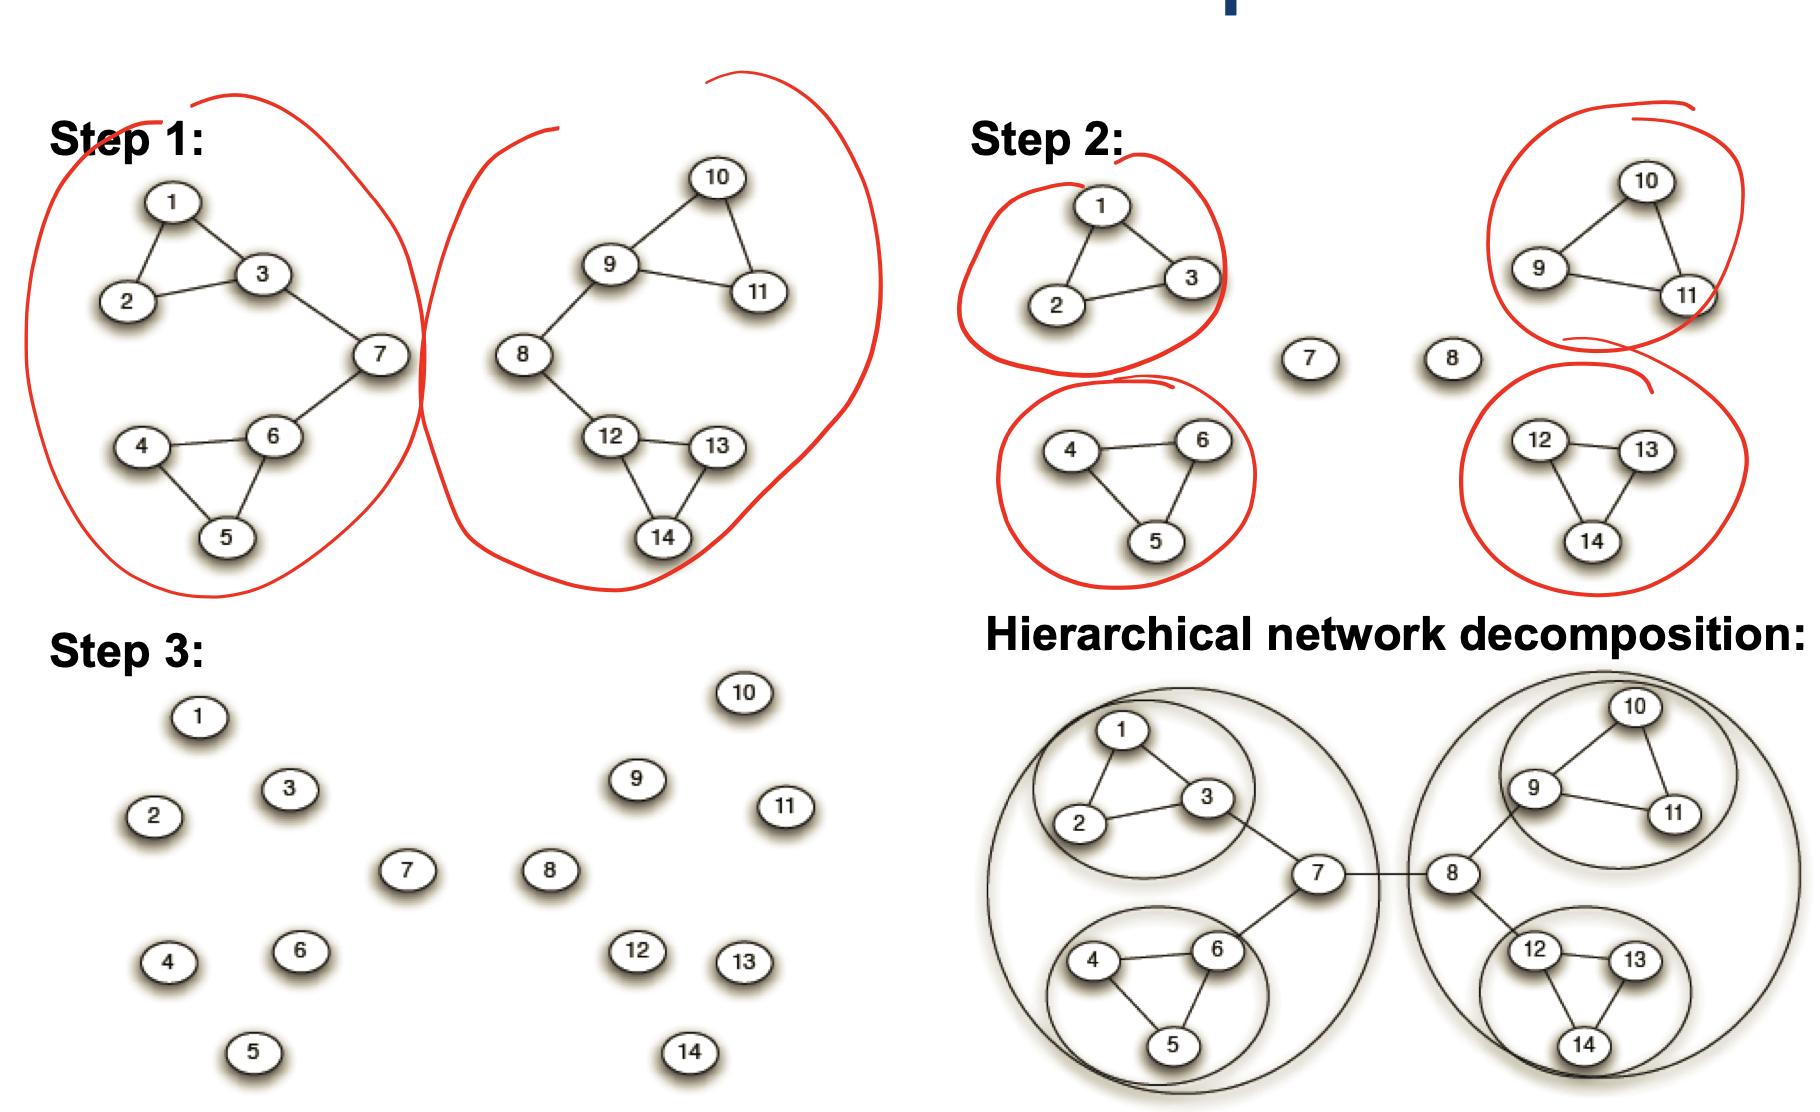
\includegraphics[width=0.5\textwidth]{images/girvandecomposition.png}
    \end{center}
    
    Betweenness can be considered a measure of the "brokerage" power of a node. the higher the betweenness, the higher the capacity the node has of acting as a broker, and the spreading of particular information. It also gives us the capacity of a graph becoming disconnected. 
    \m{
        betweenness(v) = \sum_{s \neq v \neq t}{\frac{\sigma_{st}(v)}{\sigma_{st}}}
    }
    Where $\sigma$ are the shortest paths from $s$ to $t$. By $\sigma_{st}(v))$, we mean the shortest paths from $s$ to $t$ that goes through $v$. It requires all shortest paths and requires $O(n^3)$ in the worst case. 
    
    We can use variants of Djikstra of Floyd-Warshall to count the number of shortest paths from node $A$ to all other nodes of the network. The algorithm goes as follows:
    
    \begin{itemize}
        \item Build one BFS structure for each node
        \item Determine flow values for each edge using the previous procedure (3 step)
        \item Sum up the flow values of each edge in all BFS structures to get its betweenness value. Notice we are counting the flow between each pair of nodes $X$ and $Y$ twice (once when BFS from $X$ and once when BFS from $Y$ at the end we divide everything by two.
        \item Use these betweenness values to identify the edges of highest betweenness for purposes of removing them in the Girvan-Newman method
    \end{itemize}
    
    But how do we determine number of clusters to find? Here modularity is useful for selecting the number of clusters. 
        
    \m{
        Q(G, C) = \frac{1}{2m}\sum_{c \in C}\sum_{i \in C}\sum_{j \in C}(a_{ij}- \frac{d_i d_j}{2m})
    }

\subsection{Overlapping communities}
    Nodes may participate in multiple communities at the same time. 
    
    Our first method is clique percolation. The idea is to detect densely connected communities. But first, some basic concepts
    
    \begin{itemize}
        \item $k$-clique: A complete subgraph on $k$ nodes
        \item Adjacent $k$-cliques: Two $k$-cliques that share $k-1$ vertices
        \item Community: Union of adjacent $k$-cliques
    \end{itemize}
    
\subsubsection{CFinder: Clique percolation algorithm}
    The CFinder algorithm has the following steps
    
    \begin{enumerate}
        \item Start with a $k$-clique
        \item Roll the clique over adjacent cliques. Use the adjacency criteria from before
        \item A $k$-clique community is the largest subgraph obtained by the union of all adjacent $k$-cliques. 
        \item Other $k$-cliques that can not be reached correspond to other clique-communities
    \end{enumerate}

\begin{center}
    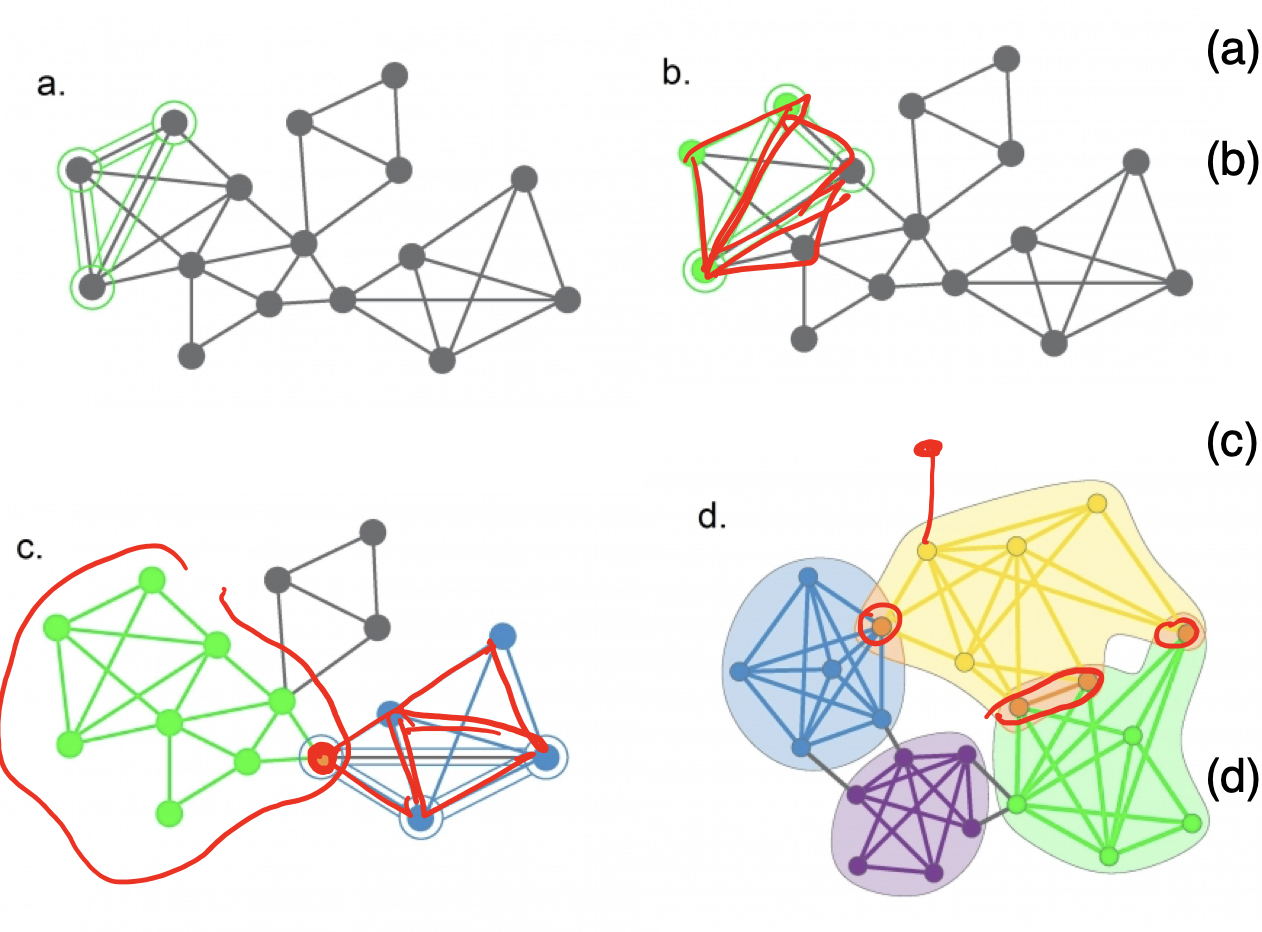
\includegraphics[width=0.5\textwidth]{images/CFinder.png}
\end{center}

Finding maximal cliques require exponential time. However the algorithm has to find only $k$-cliques, which can be done in polynomial time. 

\subsection{AGM}
    We can use a generative model for networks. Given a network, we can find the ``best'' model.  THis model will have a set of parameters that we will later want to estimate to detect communities.
    
    A question is, given a set of nodes, how do communities generate edges of the network? 
    
    If we have communities $C$, memberships $M$ and nodes $V$. Then a generative model for graphs is $B(V, C, M, \set{p_c})$. Each community has a single probability $p_c$. Later we fit the model to networks to detect communities. 
    
    For each pair of nodes in the community $A$, we connect them with probability $p_a$. The overall edge probability is
    \m{
        P(u, v) = 1 - \prod_{c \in M_u \cap M_v}{(1 - p_c)}
    }
    $M_u$ is the set of communities that node $u$ belongs to. If $u, v$ share no communities then $P(u, v) = \varepsilon$. Think of this as an OR function. If at least 1 community says yes, we create an edge.
    
    AGM can express a variety of community structures, such as non-overlapping, nested etc. 
    
\subsubsection{Maximum Likelihood Estimation for Graphs}
    Say we have that
    \begin{itemize}
        \item \textbf{Given:} Data $X$
        \item \textbf{Assumption:} Data is generated by some model $f(\theta)$
        \item We want to estimate $p_f(X | \theta)$. The probability of our model generated the data
        \item We can find the most likely model that could have generated the data, that is $\arg \max p_f(x | \theta)$
    \end{itemize}
    
    How does MLE work for graphs? Well first of all, our model generates a probabilistic adjacency matrix. We then flip all the entries of the probabilistic matrix to obtain the binary adjacency matrix. In other words, we ``flip a biased coin'' in order to determine if that should be turned on. The entries thus give the probability that two nodes are linked.
    
    The likelihood of AGM generating the graph is then
    \m{
        P(G | \Theta) = \prod_{(u, v) \in E}p(u, v) \prod_{u, v \notin E}(1 - p(u, v))
    }
    
    Our goal is then to find $\theta = B(V, C, M, \set{p_c})$ such that
    \m{
        \arg \max p(G | \Theta)
    }
    But how do we find this model? Finding $B$ means that finding the bipartite affiliation network. There is no nice way to do this. 
    
\subsubsection{From AGM to BigCLAM}
    We want to relax our problem. We say that memberships have strengths. We introduce $F_{uA}$, which is the membership strength of vertex $u$. That means that $F_{uA} = 0$. Each community $A$ links noes independently as in 
    \m{
        p_A(u, v) = 1 - \exp(-F_{uA} F_{vA})
    }
    The probability of connection is proportional to the product of the strengths. If one node does not belong to the community $(F_{uC} = 0)$ then its probability is $0$. The probability that at least one common community $C$ links two nodes is 
    \m{
        P(u, v) = 1 - \prod_{c}(1 - p_C(u, v)) = 1 - \exp(-F_u \cdot F_v^T)
    }
    We can then create a factor matrix $F$ with a column for each community, and a row for each point. Note that (80) contains the dot product. 
    
    How do we create $F$? We want to find $F$ that maximises the likelihood of 
    \m{
        \arg \max_F \prod_{u, v \in E}p(u,v) \prod_{(u, v) \notin E}(1 - p(u, v))
    }
    Where $p(u, v) = 1 - \exp(-F_u F_v^T)$. We will compute the log likelihood. (Which turns them into a sum). We want to maximize
    \m{
        l(F) = \sum_{(u,v) \in E}{log(1 - \exp(-F_u F_v^T)} - \sum_{(u,v) \notin E}F_u F_v^T
    }
    We compute the derivative of each row, and perform coordinate ascent over the rows. With caching, we can compute $F$ in linear time.
    
\subsection{Evaluating community detection}
For groups with clear definitions, such as cliques, clubs, quasi-cliques, we can verify if the extracted communities satisfy the definition.

For networks with ground truth information, we can use normalized mutual information, accuracy of pairwise community memberships etc.

When measuring cluster quality, the number of communities after grouping can be different from the ground truth. No clear community correspondence between clustering result and ground truth. NMI can then be used. 

NMI makes use of entropy. It is the information contained in a distribution.
\m{
    H(X) = - \sum_{x \in X}p(x) \log p(x)
}
Mutual information is the shared information between two distributions
\m{
    I(X; Y) = \sum_{y \in Y}\sum_{x \in X} p(x,y) \log(\frac{p(x,y)}{p_1(x)p_2(y)})
}
Normalized NMI is between $0$ and $1$ and is
\m{
    NMI(X; Y) = \frac{I(X;Y)}{\sqrt{H(X)H(Y)}}
}
    
    
    